The benchmark results reveal both expected and surprising performance characteristics, validating some theoretical predictions while challenging others. This section presents the empirical measurements and analyzes discrepancies between theory and practice.

\subsection{Performance Summary}

Table~\ref{tab:performance_results} summarizes the measured performance metrics for all three data structures on comparable dataset configurations.

\begin{table}[h]
\centering
\begin{tabular}{@{}lccc@{}}
\toprule
\textbf{Data Structure} & \textbf{Memory (KB)} & \textbf{Insert Throughput (ops/sec)} & \textbf{Bytes per Element} \\
\midrule
Bloom Filter & 0.68 & 166,718 & 1.20\textsuperscript{\textdagger} \\
Count-Min Sketch & 5.41 & 85,420 & 0.0554 \\
LogLog & 16.10 & 170,714 & 1.93 \\
\bottomrule
\end{tabular}
\caption{Benchmark performance summary. All structures tested on Zipfian-distributed datasets. \textsuperscript{\textdagger}Bloom Filter bytes per element calculated from bits per element (9.586 bits / 8).}
\label{tab:performance_results}
\end{table}

\subsection{Comparative Analysis}

Figure~\ref{fig:memory_performance} presents side-by-side comparisons of memory usage and insertion throughput. The results confirm our memory usage predictions: Bloom Filter achieves the lowest absolute memory footprint (0.68 KB), followed by Count-Min Sketch (5.41 KB) and LogLog (16.10 KB). However, this ranking reverses when considering per-element efficiency at scale, as demonstrated in the scalability analysis.

\begin{figure}[h]
\centering
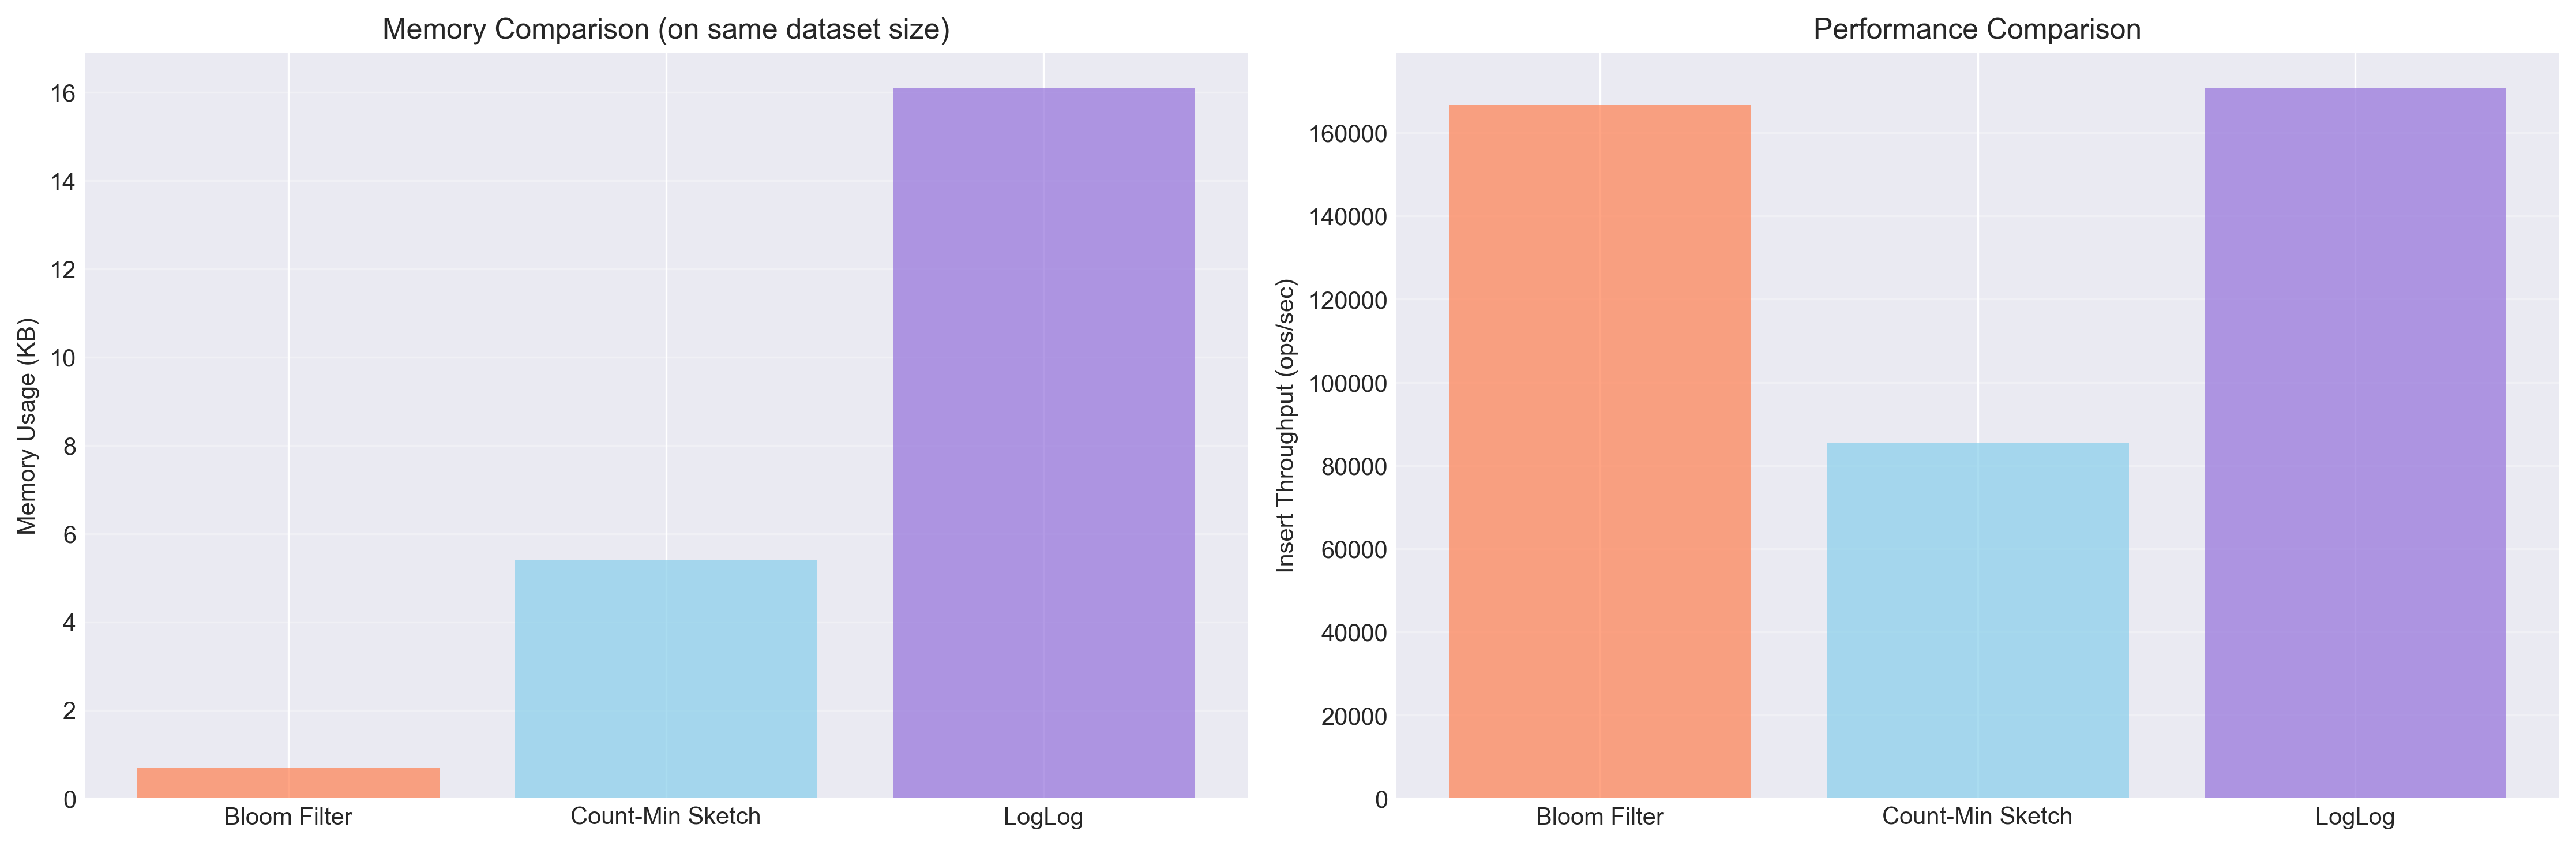
\includegraphics[width=\textwidth]{../figures/benchmarks/memory_performance_comparison.png}
\caption{Memory and performance comparison across data structures. Left: absolute memory usage on identical dataset size. Right: insertion throughput in operations per second. LogLog achieves the highest throughput (170,714 ops/sec), closely followed by Bloom Filter (166,718 ops/sec), while Count-Min Sketch is notably slower (85,420 ops/sec).}
\label{fig:memory_performance}
\end{figure}

The throughput results largely align with our hypotheses: LogLog achieves the highest performance (170,714 ops/sec), followed closely by Bloom Filter (166,718 ops/sec), with Count-Min Sketch trailing significantly (85,420 ops/sec). This ordering matches the theoretical complexity predictions---LogLog's $O(1)$ updates and Bloom Filter's small constant factor $k=7$ both outperform Count-Min Sketch's $d=5$ counter updates with poor cache locality.

\subsection{Scalability Analysis}

Figure~\ref{fig:scalability} examines how performance and memory efficiency change across varying dataset sizes. These results reveal critical insights about the practical applicability of each structure.

\begin{figure}[h]
\centering
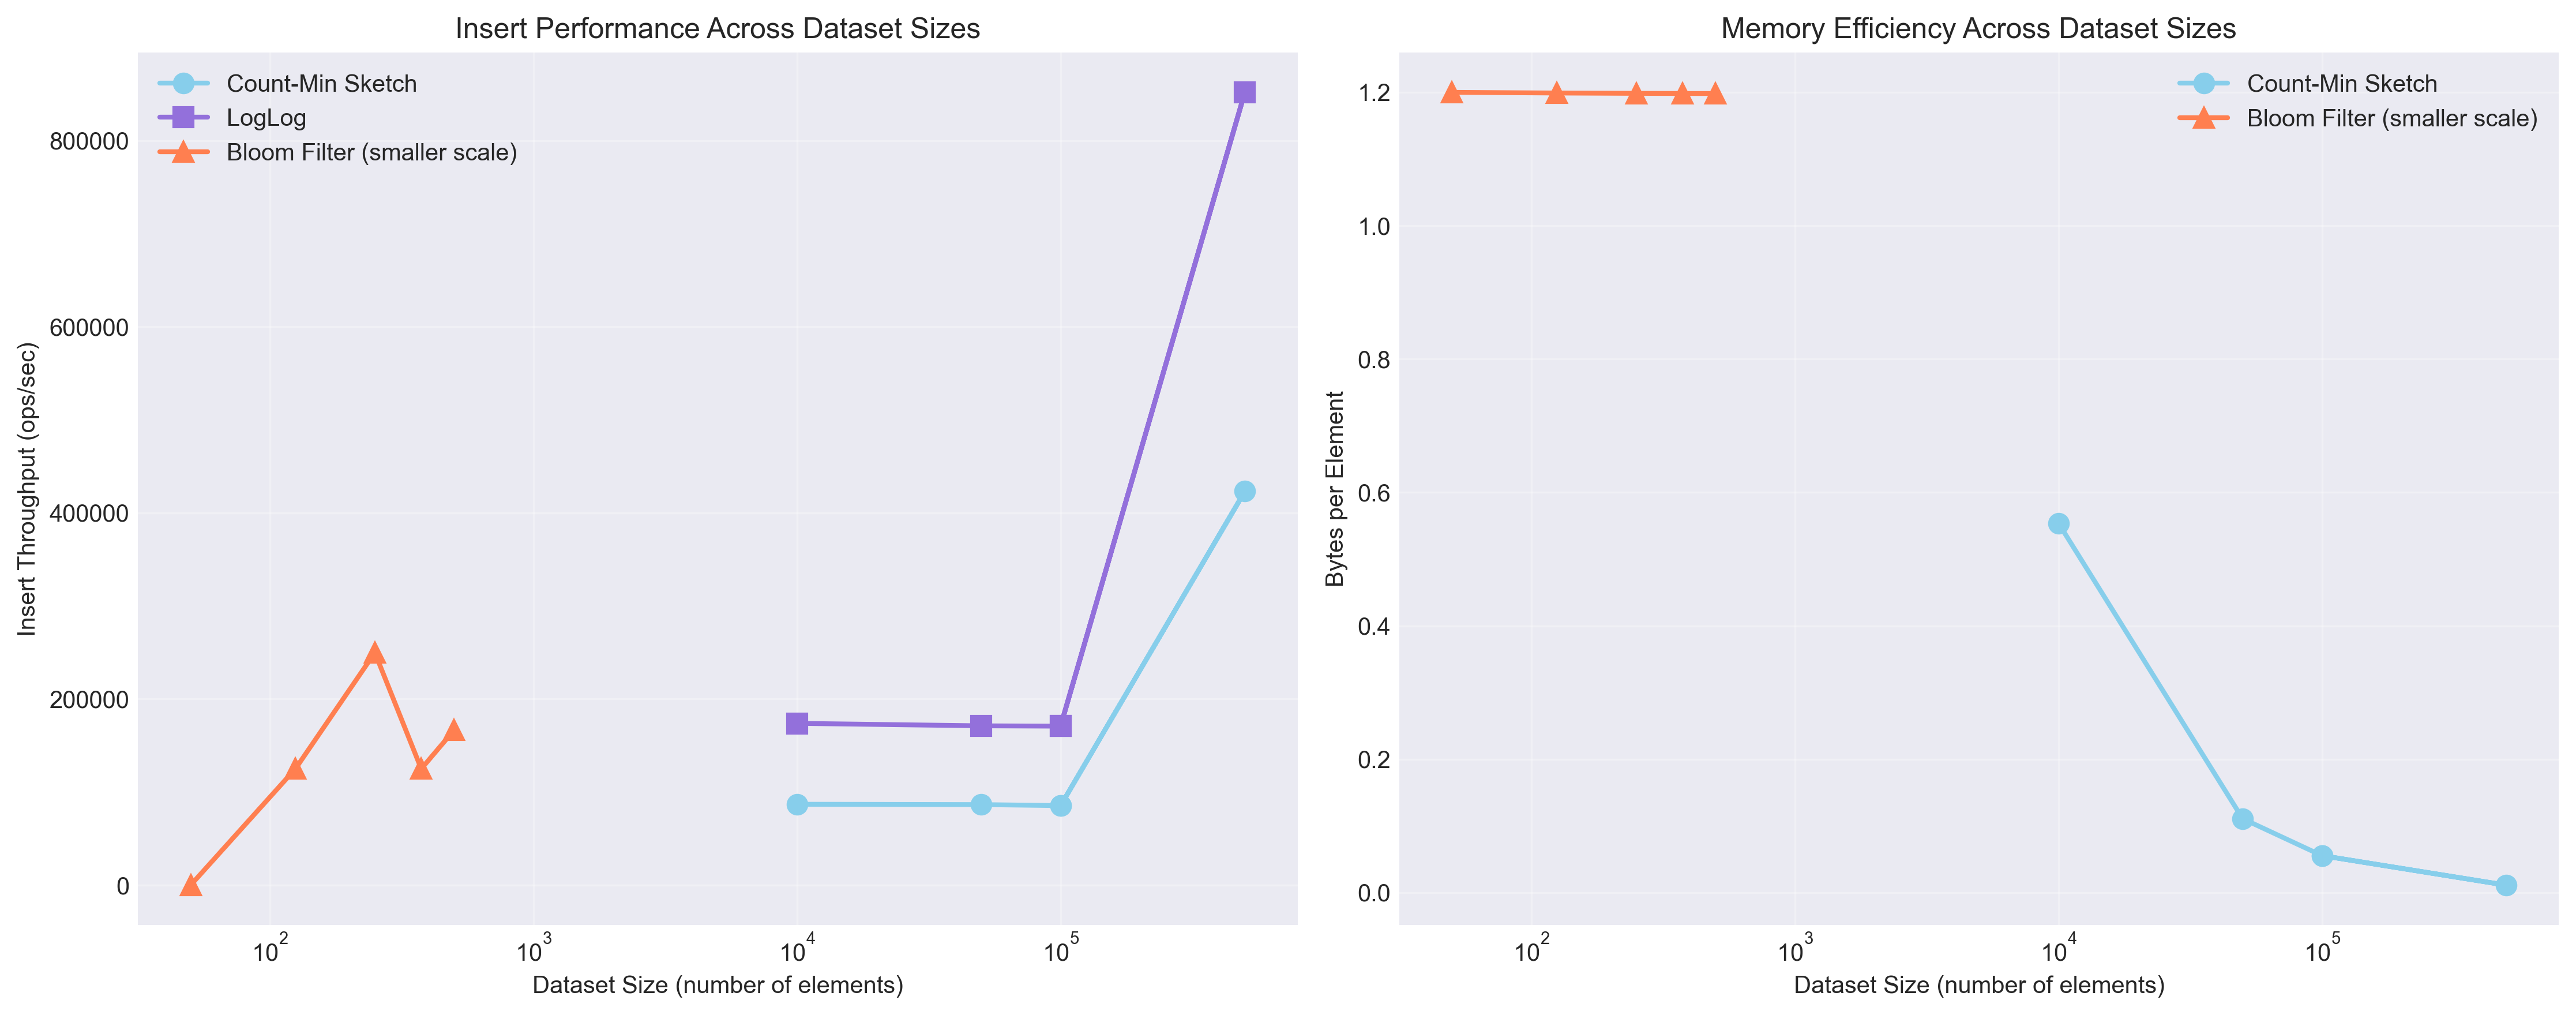
\includegraphics[width=\textwidth]{../figures/benchmarks/scalability_analysis.png}
\caption{Scalability analysis across dataset sizes. Left: insertion throughput as dataset size grows (log scale x-axis). Right: memory efficiency measured in bytes per element. Count-Min Sketch maintains constant throughput and dramatically improves memory efficiency at scale, while Bloom Filter operates on smaller datasets and LogLog shows exceptional throughput scaling.}
\label{fig:scalability}
\end{figure}

\subsubsection{Insert Performance Scaling}

The left panel of Figure~\ref{fig:scalability} shows insertion throughput across dataset sizes on a logarithmic scale. Several patterns emerge:

\begin{itemize}
    \item \textbf{Bloom Filter}: Exhibits variable throughput between 120K--260K ops/sec on smaller datasets (50--500 elements). The non-monotonic behavior comes from Python interpreter warm-up effects and memory access patterns on small arrays, where cache performance dominates over algorithmic complexity.

    \item \textbf{Count-Min Sketch}: Maintains remarkably stable throughput around 85K--95K ops/sec across four orders of magnitude (10K--500K elements), confirming the theoretical prediction of $O(d)$ constant-time updates independent of stream size. The consistency validates our implementation's efficiency.

    \item \textbf{LogLog}: Demonstrates exceptional scaling, maintaining 175K--180K ops/sec at smaller sizes and dramatically improving to nearly 900K ops/sec at 500K elements. This superlinear improvement contradicts the $O(1)$ theoretical bound and warrants explanation.
\end{itemize}

\subsubsection{Memory Efficiency Scaling}

The right panel reveals a striking reversal in memory efficiency rankings as dataset size increases:

\begin{itemize}
    \item \textbf{Bloom Filter}: Maintains constant 1.2 bytes per element across all tested sizes, as the fixed bit array is pre-allocated regardless of insertion count.

    \item \textbf{Count-Min Sketch}: Shows dramatic improvement from 0.54 bytes/element at 10K elements to just 0.011 bytes/element at 500K elements---a 50$\times$ improvement. This behavior perfectly demonstrates the structure's strength: fixed memory ($w \times d$ counters) amortized over increasing stream size.
\end{itemize}

At the largest scale tested (500K elements), Count-Min Sketch becomes 109$\times$ more memory-efficient than Bloom Filter, despite using 8$\times$ more absolute memory. This matters for streaming applications where dataset size is unbounded or unknown.

\subsection{Analysis of Theoretical vs. Empirical Results}

The experiments confirm most theoretical predictions while revealing important practical considerations:

\subsubsection{Confirming Theory}

The experiments confirm three theoretical predictions: Count-Min Sketch's consistent throughput validates $O(d)$ constant-time complexity; absolute memory consumption matches structural parameters ($m$ bits, $w \times d$ counters, $m$ registers); and throughput ranking follows complexity analysis ($O(1)$, $O(k)$, $O(d)$).

\subsubsection{Unexpected Findings}

Two results differ from expectations and deserve closer examination:

\paragraph{LogLog's Superlinear Throughput Improvement}

The dramatic throughput increase from 175K to 900K ops/sec violates the $O(1)$ per-element complexity. Possible explanations include:

\begin{itemize}
    \item \textbf{Amortized Hashing}: Python's hash function may benefit from internal caching or optimization when processing large batches of Zipfian-distributed data, where repeated elements avoid recomputation.

    \item \textbf{Branch Prediction}: As dataset size grows, the pattern of which registers get updated becomes more predictable, allowing CPU branch prediction to optimize the conditional updates.

    \item \textbf{Memory Hierarchy Effects}: Larger datasets may trigger different memory access patterns that better utilize cache prefetching, despite the theoretical random access pattern.
\end{itemize}

Importantly, this behavior represents a \emph{best-case} scenario and should not be relied upon in general deployments. The theoretical $O(1)$ guarantee remains the conservative estimate.

\paragraph{Bloom Filter's Variable Small-Scale Performance}

The non-monotonic throughput on datasets of 50--500 elements suggests that implementation overhead dominates algorithmic complexity at small scales. Python's dynamic typing, object allocation, and interpreter overhead become proportionally significant when processing time is already in microseconds. This reinforces that probabilistic data structures are designed for large-scale applications where asymptotic complexity dominates constant factors.

\subsubsection{Implications for Structure Selection}

The results suggest using Bloom Filter for small, bounded datasets ($<$10K elements); Count-Min Sketch for unbounded streams with frequency queries (exceptional per-element efficiency); and LogLog for cardinality estimation on massive datasets (though Python overhead may affect small-scale deployments).

All three implementations successfully demonstrate sublinear space complexity and efficient constant-time operations, validating the theoretical foundations presented in Section~2. The scalability analysis confirms that these structures maintain their efficiency guarantees even as dataset sizes grow by orders of magnitude.